\chapter{Konzeption}
\label{ch:Konzeption3}

Diese Kapitel beschreibt die Konzeptionsphase. Hierzu werden zu erst Anwendungsfälle definiert, um anschließend ein technisches Lösungskonzept auf Basis der Anwendungsfälle zu erarbeiten. 

\section{Definition von Anwendungsfällen}
\label{sec:Anwendungsfalle3}

\textbf{Kreditausfall-Erkennung:} Der zuerst gewählte Anwendungsfall ist das erkennen von Kreditausfällen. Ein Grund hierfür ist, dass diese Arbeit im Umfeld des Finanzsektors entsteht und somit sollen auch Anwendungsfälle aus diesem Bereich behandeln werden. Darüber hinaus besitzt das bestimmen des Kreditausfallrisikos einen sehr hohen Stellenwert innerhalb des Finanzsektors. Wie in Kapitel \ref{ch:Motivation1} bereits beschrieben, können Kredite die nicht zurückgezahlt werden zu hohen Verlusten bei Banken führen. Dies wiederum kann zu Finanzkrisen führen, die die komplette Weltbevölkerung in ihren Auswirkungen erreicht. Nichts desto trotz müssen auch die Interessen der Shareholder verfolgt werden. Daher soll ein Modell erlernt werden, dass ein Optimum zwischen Sicherheit und Gewinn gewährleistet. 

\textbf{Kreditkartenbetrugs-Erkennung:} Der Ansatz dieser Thesis soll anhand eines weiteren Anwendungsfall überprüft werden. Der zweite Anwendungsfall ist das Erkennen von betrügerischen Kreditkartentransaktionen. Studien wie \cite{FB11} zeigen, dass durch Kreditkartenbetrug in den Vereinigten Staaten im Jahr 2009, ein Schaden von 190 Milliarden Dollar entstanden ist. Ebenso zeigen Studien \cite[vgl. S. 24]{LE16}, dass im Jahr 2016 66\% aller Betrugsversuche erfolgreich sind. Aus diesem Grund wird untersucht werden, ob Machine Learning Verfahren Kreditkartenbetrug eindämmen können.   

\subsection{Erkennung von Kreditausfällen}
\label{subsec:Kreditausfallen3}

Ziel ist es Kreditanträge zu prüfen und die Ausfallwahrscheinlichkeit möglichst genau vorherzusagen. Hierzu müssen geeignete Daten verwendet werden um ein Modell zu erlernen, das die Vorhersagen treffen wird.

\subsection{Erkennung von Betrugsversuchen bei Kreditkartentransaktionen}
\label{subsec:Banktransaktionen3}

- Kurze Erläuterung von "'Fraud Detection"', sowie dessen Wichtigkeit

- Vorstellen des Datenschemas evtl. tabellarisch (Input und Output Data) 

- Vorstellen des Decision Tables

\section{Identifikation relevanter Themenfelder}
\label{subsec:Themenfelder3}

- Klären der Methodik des Prototyping um These zu beweisen

- Erläuterung des Prototypen und dessen Komponenten 
 
GRAFIK PROTOTYPE AT A GLANCE

\subsection{Basisdaten}
\label{subsec:Basisdaten3}

\textbf{Kreditausfall-Erkennung:} Nach ausgiebiger Recherche, konnten über ein Webportal der amerikanischen Hypothekenbank Fannie Mae, geeignete anonymisierte Kreditantragsdaten gefunden werden \cite{FM17}. Alle Datensätze entstammen Einfamilien-Immobilien-Dahrlehn. Die Kreditantragsdatensätze sind über Identifikationsnummern mit Performancedatensätzen verbunden, die das Zahlungsverhalten und weitere Informationen monatlich erfassen \cite{FM18}. Zum Download stehen die Acquisition- (Kreditantragsdaten) und die Performance-Datei (Performancedaten) bereit. Der erste Schritt zur Modellbildung ist die Aufbereitung der Lerndaten, diese bestehen aus Features und einem Label (vgl. \ref{sec:Machine_Learning2}).     
Als Features dienen die Kreditantragsdaten aus der Acquisition-Datei, wobei jeder Kreditantragsdatensatz mehrere Datensätze in der Performance-Datei besitzt. Aus den korrespondierenden Performancedatensätzen, muss für jeden Kreditantragsdatensatz das Label ermittelt werden. Die Kombination aus Features und Label bilden dann den Lerndatensatz. Abbildung \ref{fig:cleansing} soll den Prozess der Lerndatenerzeugung nochmals veranschaulichen.

\begin{figure}[ht]
\centering
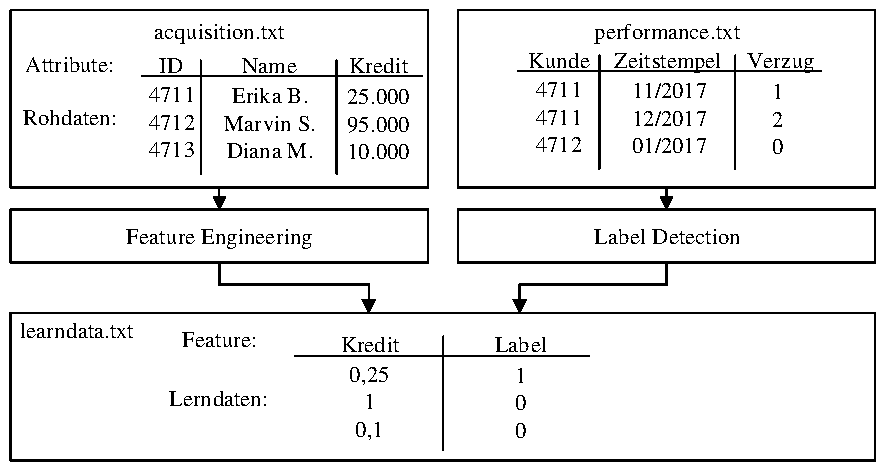
\includegraphics{images/cleansing.pdf}
\caption{Vorgehensweise bei der Erstellung des Lerndatensatzes.}
\label{fig:cleansing}
\end{figure}  

Jeder Datensatz aus der Performance-Datei stellt Informationen über Zahlungsverzüge bereit. Das Feature \textit{Current Loan Delinquency Status} beschreibt wie viele Monate der Kunde in Zahlungsverzug ist. Anhand der Identifikationsnummer wird der aktuellste Datensatz herausgesucht. Befindet sich der Kunde in Zahlungsverzug (Current Loan Delinquency Status > 0), wird dem Label der Wert 1 zu gewiesen. Liegt kein Zahlungsverzug vor wird der Wert 0 zu gewiesen. Darüber hinaus kann Current Loan Delinquency Status auch ''X'' annehmen, wenn der Zahlungsverzug unbekannt ist. Betroffenen Datensätze werden nicht zu Lerndatensätzen umgewandelt und werden übersprungen.  

\subsection{Lerndaten}
\label{subsec:Lerndaten3}

- Welche Daten werden benötigt um unser Neuronales Netz zu füttern.

- Erklärung des Erzeugungs-Algorithmus 

- Erklären von Feature Scaling

- Erklären von Labels

- Grafik mit Beispiel Datensätzen

\subsection{Evaluationsdaten}
\label{subsec:Evaluationsdaten3}

- Welche Daten werden benötigt um unser Neuronales Netz zu evaluieren.

- Erklärung des Erzeugungs-Algorithmus 

- Erklären von Feature Back Scaling

- Grafik mit Beispiel Datensätzen

\subsection{Decision-Engine}
\label{subsec:Engine3}

- Erklärung der theoretischen Funktionsweise der Decision Engine

- Erklärung des Stellenwerts innerhalb des Prototypen

\subsection{Neuronales-Netzwerk}
- Erklärung des Stellenwerts innerhalb des Prototypen 

- Funktionale Anforderungen: Lernen können sowie Datensatz evaluieren, sprich Output berechnen können

- Sollte leicht Anpassbar auf verschiedene Daten-Modelle bzw. UseCases sein 

